% !TEX TS-program = pdflatex
% !TEX encoding = UTF-8 Unicode

% This is a simple template for a LaTeX document using the "article" class.
% See "book", "report", "letter" for other types of document.

\documentclass[11pt]{article} % use larger type; default would be 10pt

\usepackage[utf8]{inputenc} % set input encoding (not needed with XeLaTeX)

%%% Examples of Article customizations
% These packages are optional, depending whether you want the features they provide.
% See the LaTeX Companion or other references for full information.

%%% PAGE DIMENSIONS
\usepackage{geometry} % to change the page dimensions
\geometry{a4paper} % or letterpaper (US) or a5paper or....
% \geometry{margin=2in} % for example, change the margins to 2 inches all round
% \geometry{landscape} % set up the page for landscape
%   read geometry.pdf for detailed page layout information

\usepackage{graphicx} % support the \includegraphics command and options
\usepackage[parfill]{parskip} % Activate to begin paragraphs with an empty line rather than an indent

%%% PACKAGES
\usepackage{booktabs} % for much better looking tables
\usepackage{array} % for better arrays (eg matrices) in maths
\usepackage{paralist} % very flexible & customisable lists (eg. enumerate/itemize, etc.)
\usepackage{verbatim} % adds environment for commenting out blocks of text & for better verbatim
\usepackage{subfig} % make it possible to include more than one captioned figure/table in a single float
% These packages are all incorporated in the memoir class to one degree or another...

%%% HEADERS & FOOTERS
\usepackage{fancyhdr} % This should be set AFTER setting up the page geometry
\pagestyle{fancy} % options: empty , plain , fancy
\renewcommand{\headrulewidth}{0pt} % customise the layout...
\lhead{}\chead{}\rhead{}
\lfoot{}\cfoot{\thepage}\rfoot{}

%%% SECTION TITLE APPEARANCE
\usepackage{sectsty}
\allsectionsfont{\sffamily\mdseries\upshape} % (See the fntguide.pdf for font help)
% (This matches ConTeXt defaults)

%%% ToC (table of contents) APPEARANCE
\usepackage[nottoc,notlof,notlot]{tocbibind} % Put the bibliography in the ToC
\usepackage[titles,subfigure]{tocloft} % Alter the style of the Table of Contents
\renewcommand{\cftsecfont}{\rmfamily\mdseries\upshape}
\renewcommand{\cftsecpagefont}{\rmfamily\mdseries\upshape} % No bold!


\usepackage{algorithmicx}
\usepackage{algpseudocode}


%%% END Article customizations

%%% The "real" document content comes below...

\title{Project Final Report}
\author{Jiachi Liu \& Peili Cao}
%\date{} % Activate to display a given date or no date (if empty),
         % otherwise the current date is printed 

\begin{document}
\maketitle

\section{Introduction}
Music recommendation is a core feature for current online music applications. In this project, we implemented two data mining algorithms to recommend music to users. K-Means algorithm is used to recommend similar musics whereas frequent itemsets mining will find the combination of songs that most user will listen together.

\subsection{K-Means}
K-Means algorithm is a popular clustering algorithm aims to partition n data points into K clusters which each data point belongs to the cluster with the nearest mean. And it is also a unsupervised machine learning algorithm since the data points usually without labels. In this project, a Distributed version of KMeans algorithm is implemented with MapReduce to partition the millionSongs dataset into different clusters. Thus in future, given a new song data point, we can find the similar songs based on the clusters and recommend it to the user.

\section{Data}
\subsection{K-means}
For K-Means major task, we are using MillionSongs dataset to divide songs into K different clusters. Since million songs dataset contains a lot of meta data of music, such as mode, key, segments, we are using a subset of those features to reduce the size of data, which contains 15 features. The features are: artist familiarity, artist hotness, number of similar artists, number of artist terms, duration, end of fade in, key, key confidence, loudness, mode, mode confidence, start of fade out, temp, year, song hotness. Figure \ref{fig:msd} shows some lines of data as example.

Since the entire data set is very large, we are using a subset of million songs dataset which contains 10000 songs in H5 format files. This subset can be found at 

http://labrosa.ee.columbia.edu/millionsong/pages/getting-dataset

In order to extract features from H5 file, we wrote a small java program to read the data from this format. The source code is under extractFeatures package and hdf5\_getters.java is the official library to parse the H5 file.

\begin{figure}[htbp]
\begin{center}
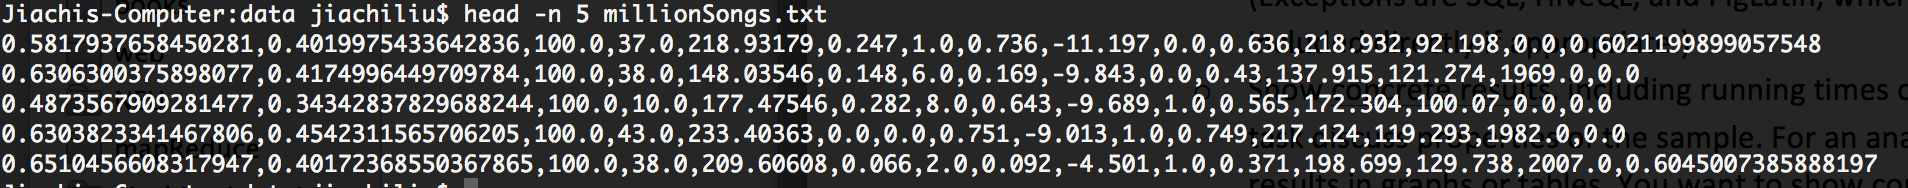
\includegraphics[scale=0.4]{millionsongs.png}
\caption{Million Songs data example}
\label{fig:msd}
\end{center}
\end{figure}

\section{Technical discussion}
\subsection{K-Means}
For K-Means task, we have implemented both distributed and local version of KMeans algorithm. Our goal is to split the given songs into K different clusters based on selected features and get the centroid for each cluster. For local algorithm, parallel computing is applied to explore different K at same time. Both distributed and local algorithm will output the final centroids into file which can be used to assign data point to corresponding clusters. 

\subsubsection{Distributed KMeans}
The Mapper of KMeans Algorithm will read the current K centroids from HDFS file and save them into the memory in setup function. In map function call, for each line of data, we assign it to the centroid that has minimum distance. The distance is calculated as Euclidean distance between the data point and centroids. The mapper then emits the centroid id as a key and the data point as value.

\begin{algorithmic}[1]
\Function{map}{key, data}
\State $minDistance \gets Infinity$
\State $centroidId = -1$
\For{each centroid $c$ in centroids}
	\State $dist \gets distance(c, data)$
	\If{$dist < minDistance$}
		\State $minDistance \gets dist$
		\State $centroidId = c.id$
	\EndIf
\EndFor
\State $emit(centroidId, data)$
\EndFunction
\end{algorithmic}

The reducer will update the centroid vector by calculating the average vector among the input data point list. And emit the new centroid to output file.
\begin{algorithmic}[1]
\Function{reduce}{cid, [$d_1,d_2....,d_n$]}
\State $sumVector \gets 0$
\State $count \gets 0$
\For{each data $d$ in input list}
	\State $sumVector +=  d$
	\State $count ++$
\EndFor
\State $newCentroid = sumVector / count$
\State $emit(newCentroid, Null)$
\EndFunction
\end{algorithmic}

The Driver class will repeatedly create map reduce job for each iteration of KMeans. And it will set the number of reducers as same as K. It will first initialize centroids based on input K before start KMeans algorithm, and then start create jobs for each iteration to get new computed centroids. After that, it will copy the output file to currentCentroid folder so the mapper can read current centroids from it. Also, it will delete the output file in order to avoid exceptions on map reduce job. And to stop the iterations, it will read and compute the sum of distance of all centroids between two iterations and determines whether to stop.

The following pseudo code shows the process of driver program:
\begin{algorithmic}[1]
\Function{train}{Input arguments}
\State read the dataset file path, current centroid file path, and new centroid file path from program input arguments.
\State read K from input arguments
\State init K centroids from dataset and write them to new centroid file.
\While{Not converge}
	\State copy the new centroid file to current centroid file
	\State delete the new centroid file
	\State run map reduce job on current centroid file and input dataset to get new centroid file
\EndWhile

\EndFunction
\end{algorithmic}

The following pseudo code shows the logic on determining converge. This program will read new centroids and current centroids from S3 that output by map reduce jobs.

\begin{algorithmic}[1]
\Function{isConverge}{oldCentroids, newCentroids}
\State $dist \gets 0$
\For{each old centroids o, and new centroids n}
	\State $dist += distance(o, n)$
\EndFor \\
\Return $dist <= threshold$
\EndFunction
\end{algorithmic}

The source code related to Distributed KMeans algorithm is shows as following:
\begin{itemize}
\item KMeansMapReduce.java the map reduce job
\item KMeansController.java the driver program
\item DenseVector.java the vector class to compute the distance
\item FileReadWriteUtil.java helper class for file read, write, delete and copy
\end{itemize}

\subsubsection{Distributed KMeans - Running Result}
Table \ref{table: kmean-running-time-table} shows the running time of Distributed KMeans on AWS for different K. We are using two configurations, one is 5 small machine and one is 10 small machines.

\begin{table}[htdp]
\caption{K-Means Runtime Table}
\begin{center}
\begin{tabular}{|c|c|c|c|}
\hline
K & \# of Iterations & 5 workers & 10 wokers\\ \hline
2 & 2 &	4m01s & 3m32s \\ \hline
3 & 11 &	21m43s & 20m41s\\ \hline
5 &	18 & 38m32s & 34m38s\\ \hline
10 & 32 & 1h09m12s & 1h00m33s	\\ \hline
20 & 58 & 2h30m41s & 2h00m07s	\\ \hline
30 & 76 & 3h52m58s & 2h56m49s	\\ \hline
\end{tabular}
\end{center}
\label{table: kmean-running-time-table}
\end{table}%

\begin{figure}[htbp]
\begin{center}
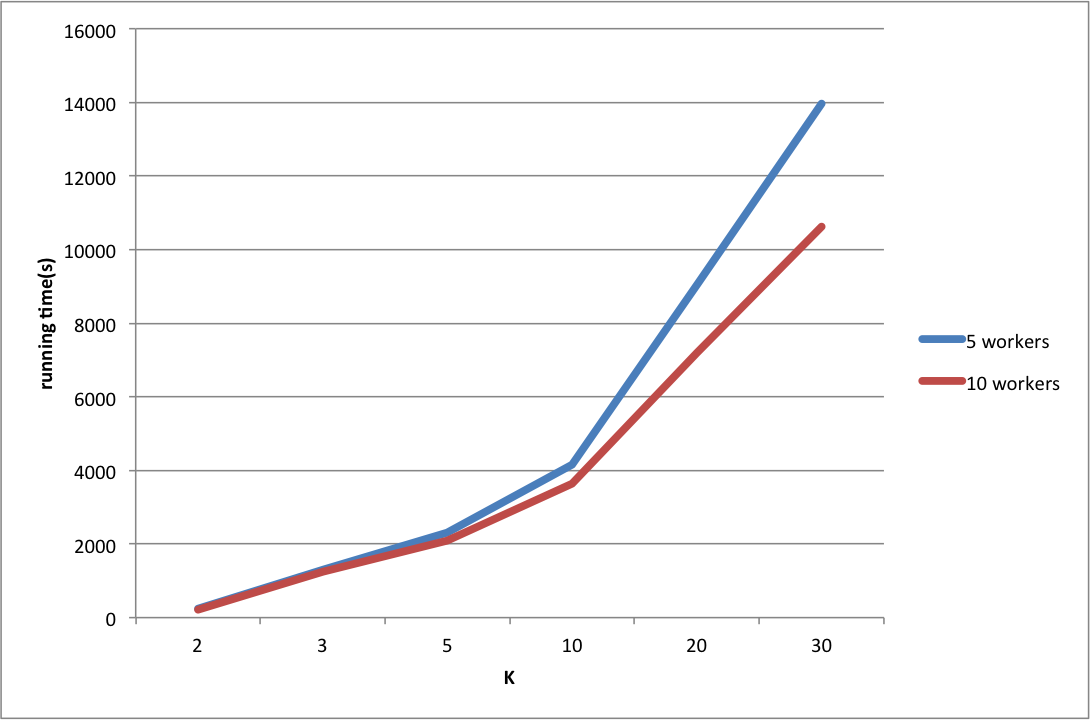
\includegraphics[scale=0.7]{dkmeans-runtime.png}
\caption{Distributed KMeans - Running Time}
\label{fig:dkmeans-runtime}
\end{center}
\end{figure}

\begin{figure}[htbp]
\begin{center}
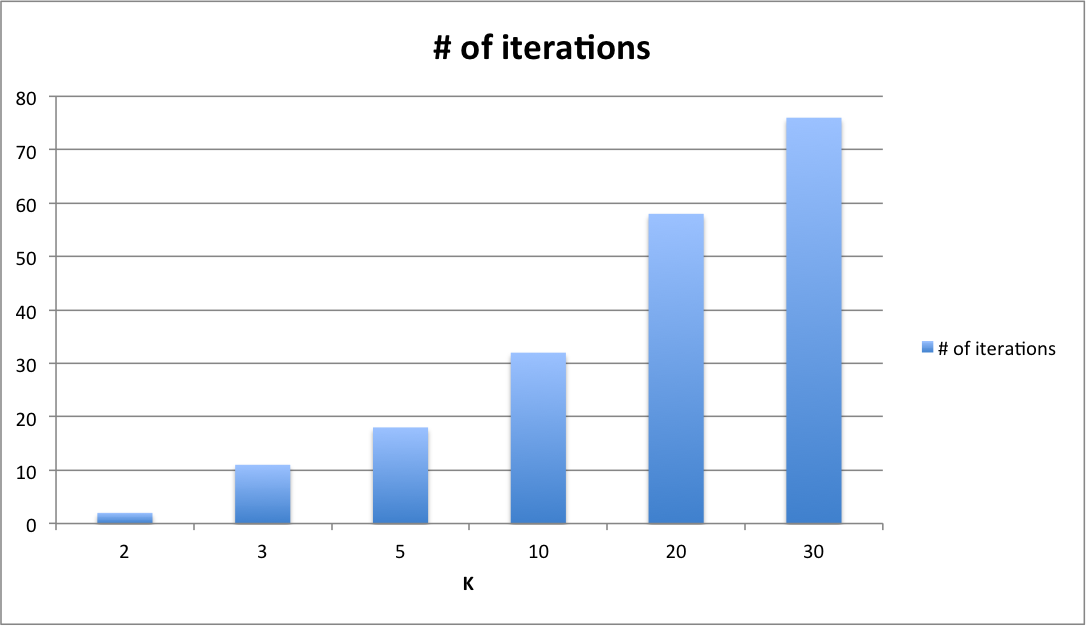
\includegraphics[scale=0.7]{kmeans-iter.png}
\caption{KMeans - Number of Iterations with Different K}
\label{fig:kmeans-iter}
\end{center}
\end{figure}


As the table shows, under same configuration, with the increasing number of K, the total number iterations is also increased and thus more time is needed to finish the algorithm. However, when we double the worker machines, the running time is not decreased to half as we expected. Based on the algorithm introduced above, the number of reducers is same as the K values. When K is small, not all workers is computing the new centroid during reduce phase. Thus the running time is almost same when K is 2,3,5,10. But when K becomes larger, for instance 30, it is possible for all reducers participated in computing thus less time is needed.

\subsubsection{Local KMeans with MapReduce}
We also implemented local version of KMeans algorithm and running multiple K-s with mapreduce. The basic idea is that each mapper running the local version KMeans to get the final centroids. And NLineInputFormat is used in order to let different mapper handle different K in input file. For this problem, the input data is a file that each line is a single number that represents a value of K. The dataset will be put in Distributed Cache and load into memory during the map phase, since the size of dataset can be fit into memory.

The following pseudo code shows the local KMeans algorithm:
\begin{algorithmic}[1]
\Function{local KMeans}{input dataset, K}
\State init K centroids from input dataset
\While{True}
\For{each data t in dataset}
	\State find the closest centroid c from centroids
	\State assign t to cluster respect to c
\EndFor
\For{each cluster cl}
	\State calculate the new centroid from data point that assigned to cl
	\State add new centroid to new centroid list
\EndFor
\If{Converge(newCentroids, currentCentroids)}
	\State break
\EndIf
\EndWhile
\EndFunction
\end{algorithmic}

Mapper pseudo code is shows as following. The input value is the  parameter K which is also used as output key to distinguish different centroids from mapper output.

\begin{algorithmic}[1]
\Function{map}{key, value}
\State read dataset from distributed cache to memory
\State run local KMeans algorithm on dataset and get the centroids
\For{for each centroid c in centroids}
	\State emit(value, c)
\EndFor
\EndFunction
\end{algorithmic}

Reducer pseudo code is shows as following. The reducer will collect all centroids from the current K and emit it to output file.
\begin{algorithmic}[1]
\Function{reduce}{key, values}
\State read dataset from distributed cache to memory
\State run local KMeans algorithm on dataset
\For{each value in values}
	\State emit(key, value)
\EndFor
\EndFunction
\end{algorithmic}

\subsubsection{Local KMeans - Running Result}
We also apply two configurations(5 workers and 10 workers) for this problem and set the converge condition as same as distributed version. The input file contains 6 different K, which is 2,3,5,10,20,30. For 5 workers, it took 2min31s to finished the job. For 10 workers, it took 2min37s. The running time is not change accordingly with number of workers. Due to the NLineInputFormat, the number of mappers is fixed during the execution thus increasing the number of machines will not have significant different on running time when input parameters is small. 

\subsubsection{Local KMeans v.s. Distributed KMeans}
Now comparing with distributed version, local version took much smaller time to finished the job. The reason is that:
\begin{itemize}
\item Distributed version KMeans repeatedly setup new job for each iteration. On AWS, job setup takes a lot of time which heavily extend the total execution time. Where the local version only have one job to setup.
\item The local version only send final centroids from mapper to reducer one time, whereas distributed version needs to send the entire dataset in each iteration. The data transition between the mapper and reducer also takes time. This can be verified from the log file. Figure \ref{fig:syslogk3} shows one iteration of Distributed KMeans when $K=3$, we can see that the total number of mapper output is 10000 which is the entire dataset. And Figure \ref{fig:sysloglocal} shows the local version of KMeans mapper output is 70, which is the sum of all different numbers of K in NLineInput file.
\item Distributed version also needs to copy and read centroids from S3 file, where local version finished everything in memory.
\end{itemize}

\begin{figure}[htbp]
\begin{center}
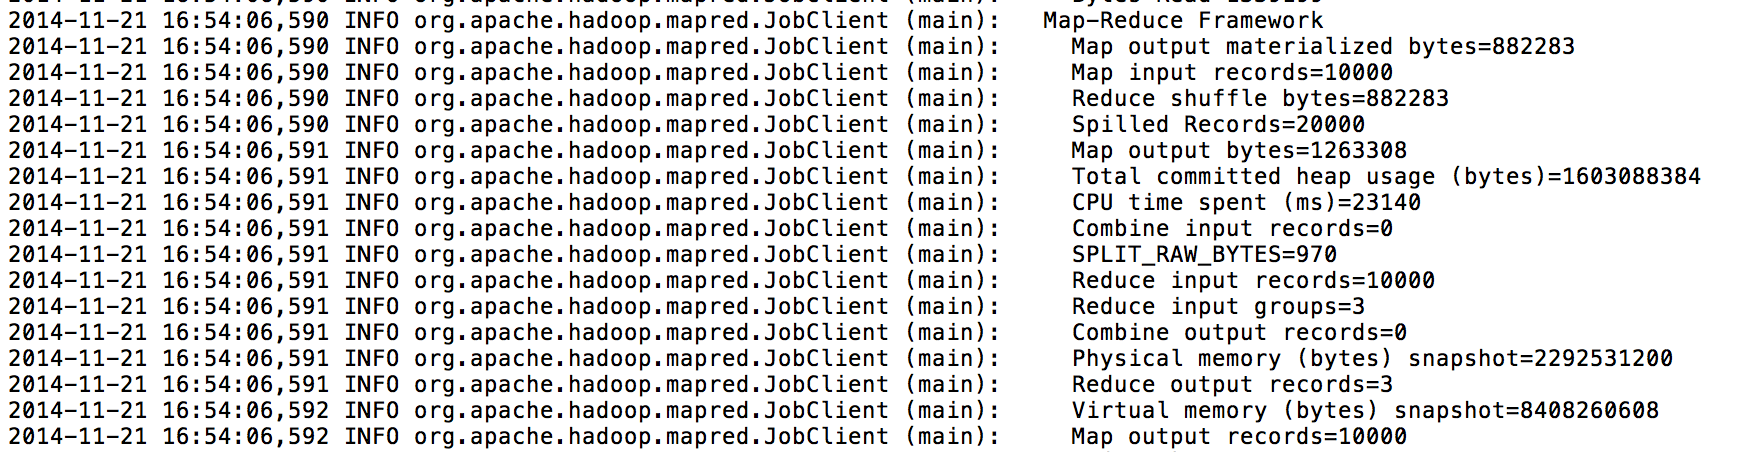
\includegraphics[scale=0.4]{syslogk3.png}
\caption{Syslog for Distributed Version KMeans - K=3}
\label{fig:syslogk3}
\end{center}
\end{figure}

\begin{figure}[htbp]
\begin{center}
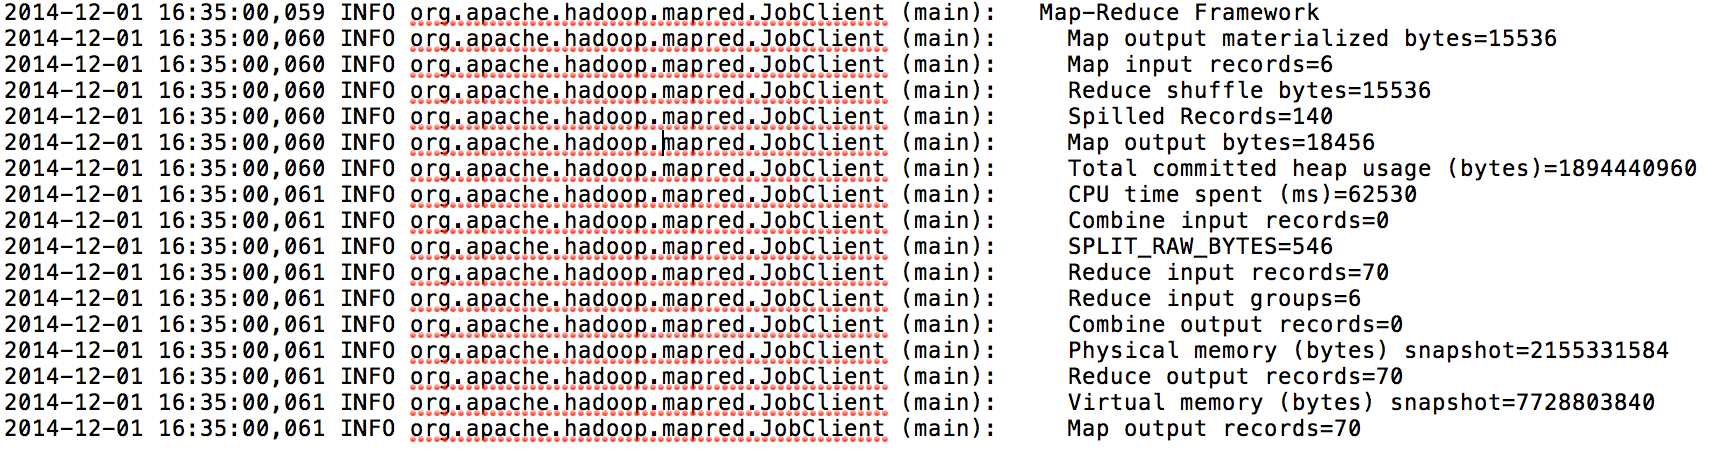
\includegraphics[scale=0.4]{sysloglocal.png}
\caption{Syslog for Local Version KMeans}
\label{fig:sysloglocal}
\end{center}
\end{figure}

The source code for local version is also in DistributedKMeans folder, which contains LocalKMeans.java, LocalKMeansController.java and KMeansLocalMapReduce.java.

\section{Conclusion}
\subsection{K-Means}
Local version of K-Means is much faster than distributed version in our experiments. However, our implementation of local version is loading the dataset into memory which may not feasible in practical problems. For distributed version, the job setup takes a lot of times compare with the actual computing time, a better way should be found to avoid repeatedly create jobs in each iteration.

Another issue for distributed K-Means is that we need to save the generated centroids to some where and also keep tracking the old centroid generated in last iteration. In our implementation, we copy the new centroids file to other place and read it back when checking the converge condition, which also requires additional time.

In order to compare the performance of two implementation, we fixed the initial centroids and converge condition to ensure the number iteration is same in both distributed version and local version. However, practically, the initial centroids should be carefully determined since KMeans algorithm is very sensitive with the start points. And in order to reduce the number of iterations, the initial centers should be as far as possible to each other. In future work, a carefully designed algorithm, such as Furthest First Traversal, should be applied to find the optimal initial centers.

\end{document}

